\begin{frame}
	\frametitle{Produto}
	
	\begin{center}
		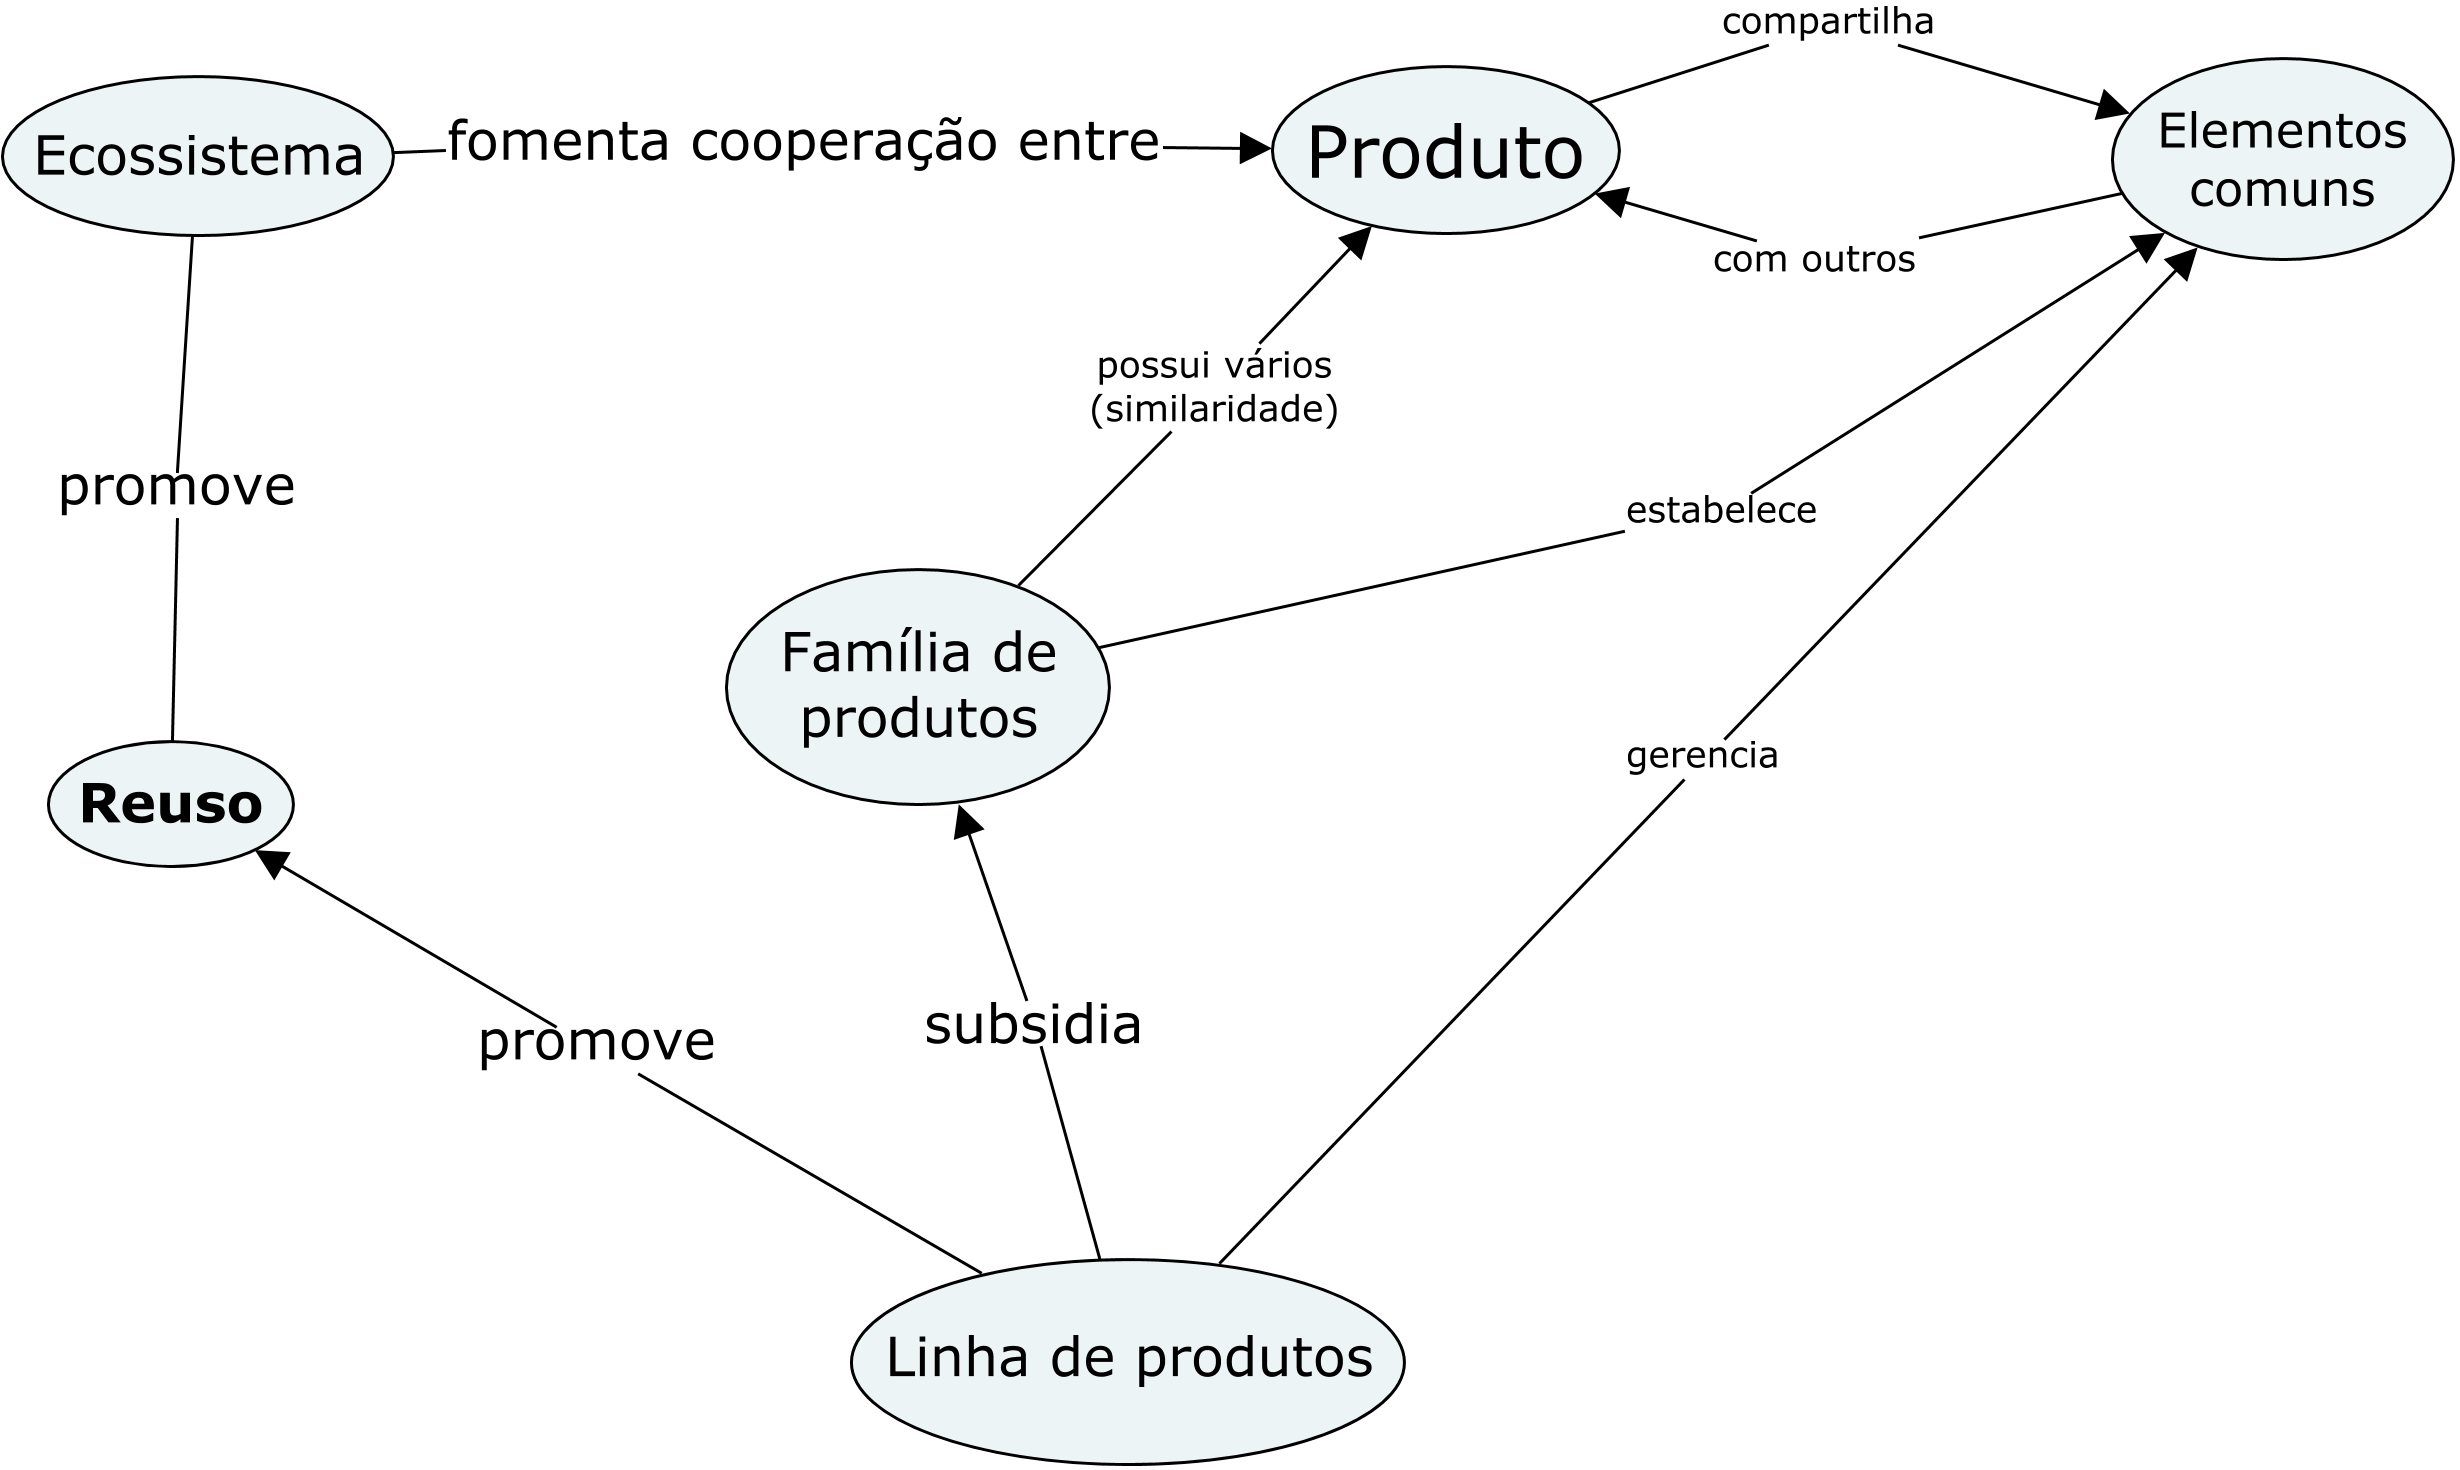
\includegraphics[width=\textwidth]{product-family-ecosystem}
	\end{center}
\end{frame}



\section{Gerenciamento}

\begin{frame}
	\frametitle{Gerenciamento de produto}

	\begin{block:concept}{Gerenciamento de produto}
		Gerenciamento de produto é a disciplina e o processo de negócio
		que governa o produto desde sua concepção para o mercado até sua
		entrega e retirada, trazendo o maior valor possível para o
		negócio da empresa.
	\end{block:concept}

	\begin{block:fact}{Principais grupos de processos}
		\begin{itemize}
			\item Gerenciamento de portfólio.
			\item Marketing do produto.
			\item Desenvolvimento do produto.
		\end{itemize}
	\end{block:fact}
	
	\note{
		\begin{itemize}
			\item Gerenciamento de produto bem sucedido significa a entrega do
			produto certo na hora certa para o mercado certo.
			
			\item Falar da experiência no NUMA: integração de aplicações técnicas (computação),
			gerenciamento (engenharia de produção) e negócio (relacionamento com clientes) no
			contexto de software livre.		
			
			\item Fazer o gancho para todas as atividades feitas e que constam no próximo slide.
		\end{itemize}
	}
\end{frame}



% \begin{frame}
% 	\frametitle{Gerenciamento de produto (software)}
% 	\framesubtitle{Produto X Projeto: Grupo de processos}
% 
% 	\begin{block:fact}{}
% 		\centering
% 		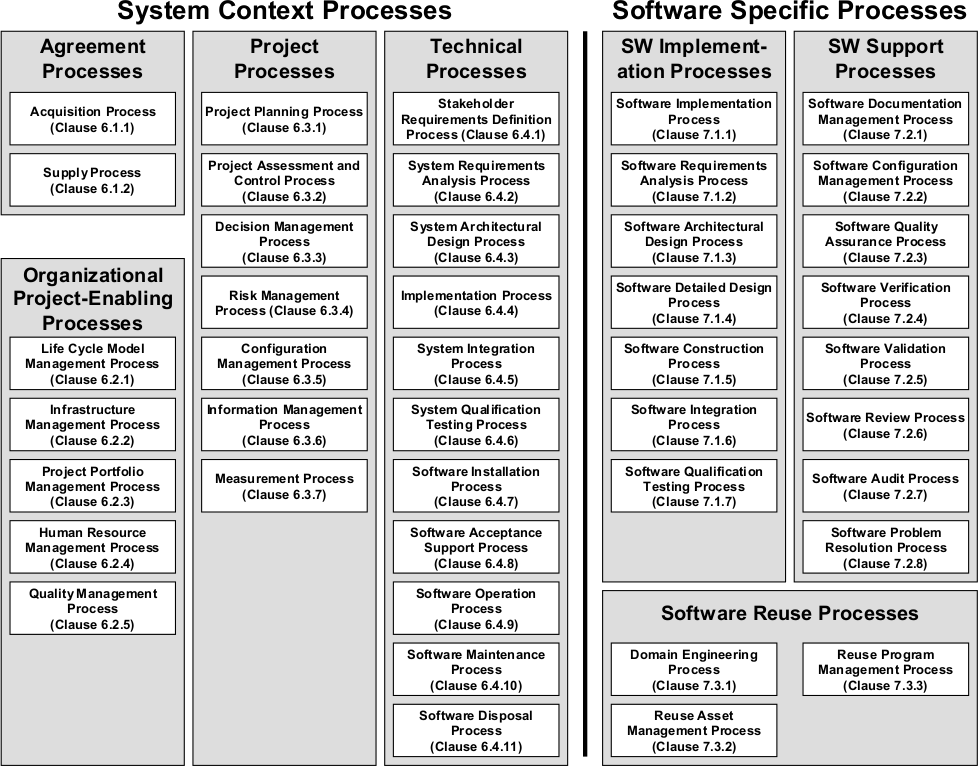
\includegraphics[width=\textwidth]{software-engineering/project-management/product/iso12207}
% 	\end{block:fact}
% 	
% 	\note{
% 		The ISO life cycle related standards for systems life cycle
% 		processes (ISO/IEC 15288:2002, 2002) and software life
% 		cycle processes (ISO/IEC 12207:1997, 1997) primarily look
% 		into the processes from analysis to development to distri-
% 		bution and further downstream towards operations and
% 		even disposal. They do not detail the upstream activities
% 		before project start or product launch.
% 	}
% \end{frame}

\begin{frame}
	\frametitle{Gerenciamento de produto (software)}

	\begin{block:fact}{\small Arcabouço de referência para gerenciamento de produtos (software)}
		\centering
		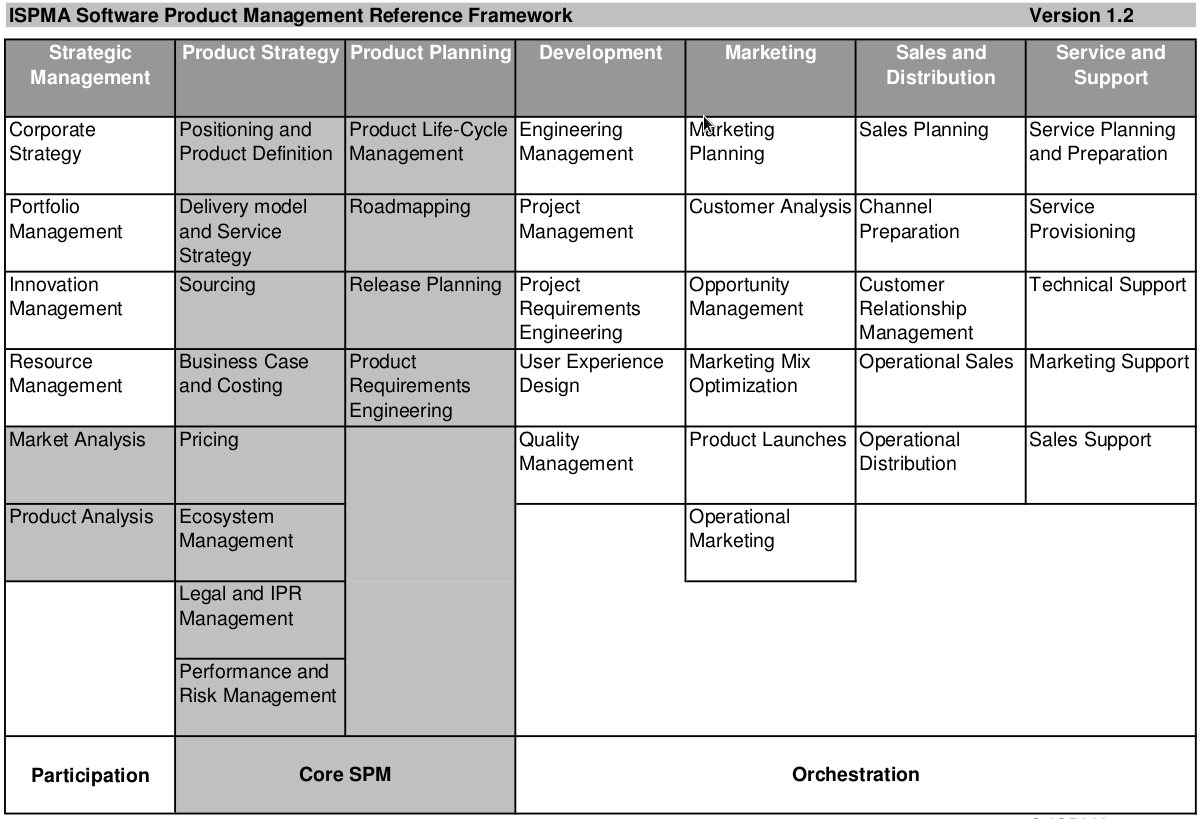
\includegraphics[width=\textwidth]{software-engineering/project-management/product/ispma}
	\end{block:fact}
	
	\note{
		\begin{itemize}  
			\item Market analysis and product analysis are the sources of the raw
			qualitative and quantitative decision-making data for the product manager.
		 
			\item Product strategy and product planning are the business-oriented core
			functions of product management.
		 
			\item The other functions (development, marketing, sales and
			distribution, support and services) are not directly related to the
			tasks of the product manager and thus he needs to collaborate
			with the respective departments about decisions concerning these
			functions.
		\end{itemize}
	}
\end{frame}


\subsection{Escopo}

\begin{frame}
	\frametitle{Gerenciamento de produto (software)}
	\framesubtitle{Escopo}
	
	\begin{block:concept}{Escopo}
		Definição de escopo é o processo de dividir objetivos ou requisitos
		de um produto e de um projeto em partes menores e mais concisas.
	\end{block:concept}


	\begin{block:fact}{Escopo}
		\begin{center}
			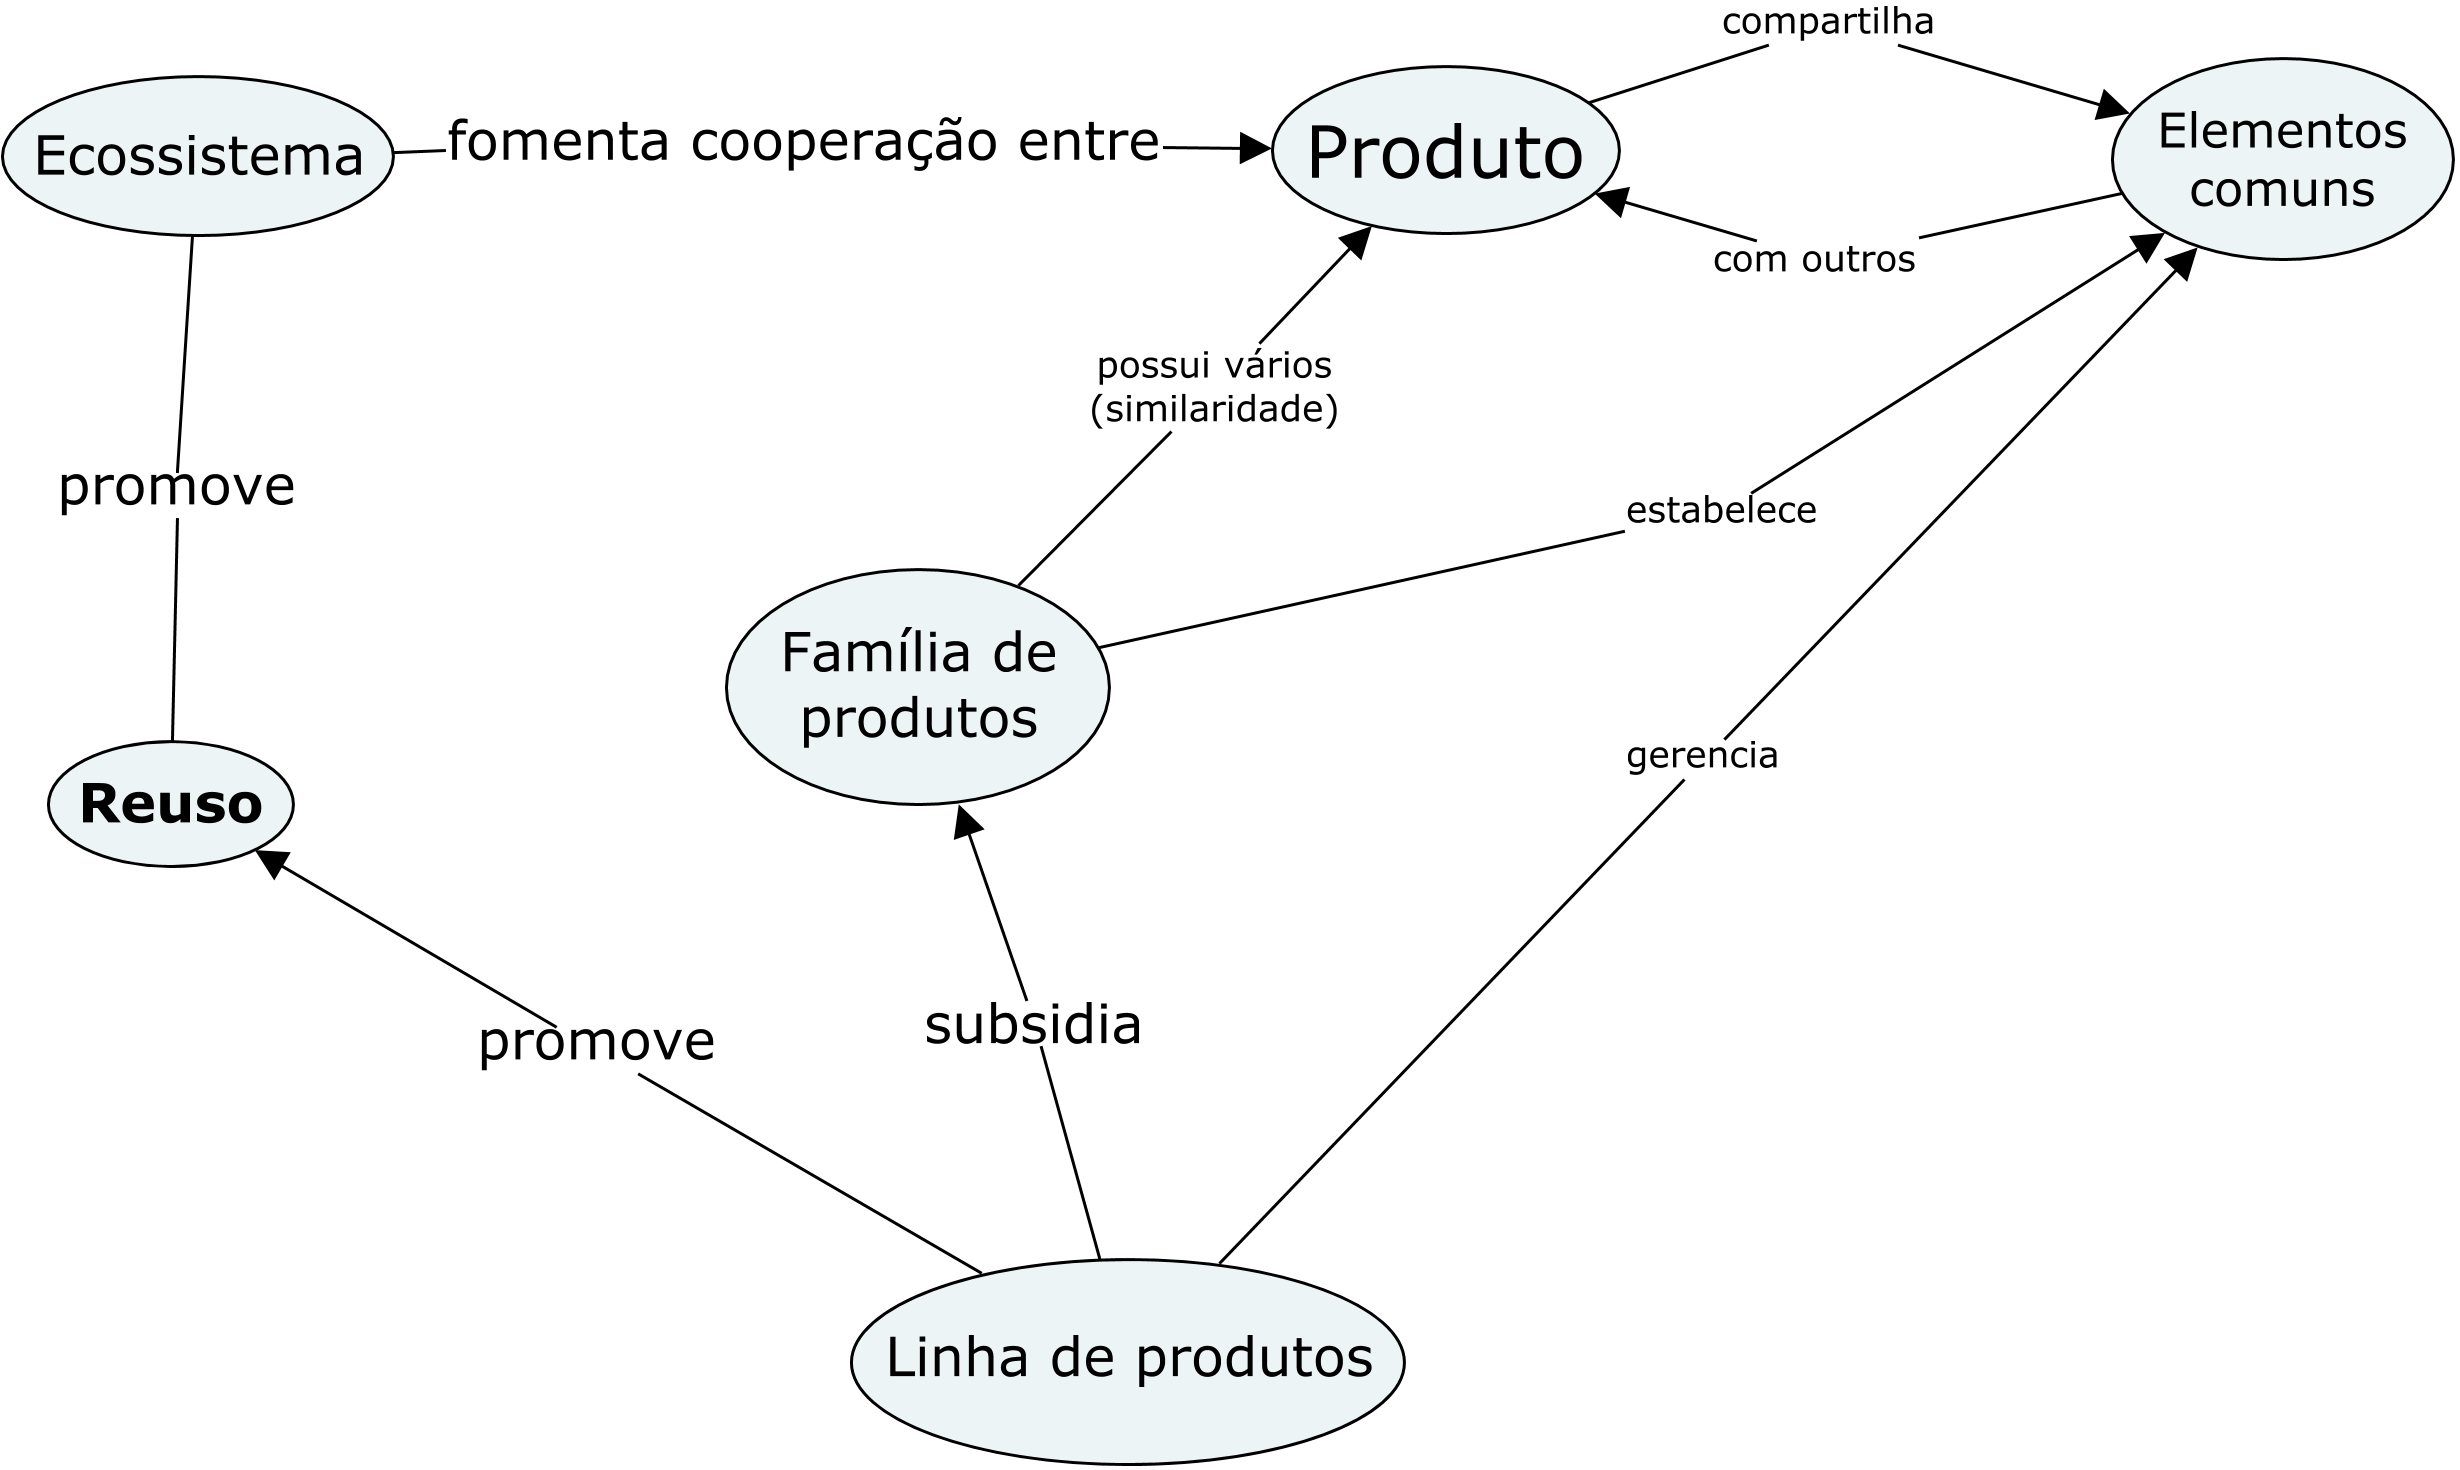
\includegraphics[width=.8\textwidth]{product-family-ecosystem}
		\end{center}
	\end{block:fact}
	
	\note{
		Breve história de evolução:
		\begin{itemize}
			\item Primeiros sistemas computacionais: software + hardware, totalmente integrados.
			
			\item IBM + MS-DOS
			
			\item Windows
			
			\item Web (mashups, serviços Web)
			
			\item Aplicações para dispositivos móveis (appstores)
		\end{itemize}
		
		Escopo cada vez mais reduzido, o que também proporciona a definição de mais produtos e projetos!
		
		Ecossistemas: preocupação em oferecer bons serviços comuns a diversas aplicações diferentes.
	}
\end{frame}


\begin{frame}
	\frametitle{Gerenciamento de produto (software)}
	\framesubtitle{Escopo: Produto X Projeto}
	
	\begin{block:fact}{Escopo do \textbf{produto}}
		\begin{itemize}
			\item Tendências de mercado
			\item Requisitos de cliente
			\item Interesses da empresa ou comunidade (lucro, aumento de participação/visibilidade)
		\end{itemize}
	\end{block:fact}
	
	\begin{block:fact}{Escopo do \textbf{projeto}}
		\begin{itemize}
		 	\item Entrega do projeto na data correta,
		 	
		 	\item Cumprimento do orçamento estabelecido.
		 	
		 	\item Satisfação de requisitos de qualidade.
		\end{itemize}
	\end{block:fact}

	\note{
		\begin{itemize}
			\item Produto: voltado para o lançamento e criação.
			
			\item Projeto: voltado o desenvolvimento, manutenção.
			
			\item Atualmente é possível uma relação quase 1 para 1 entre produto e projeto em alguns segmentos,
			ou seja, lançar um produto distinto a cada projeto.
		\end{itemize}
	}
\end{frame}


\subsection{Proteção intelectual}


\begin{frame}
	\frametitle{Proteção intelectual}
	
	\note{
		Gestão das propriedades intelectuais:
		\begin{itemize}
			\item Quais são? Direitos autorais (copyright), segredo industrial e patentes. Explicar
			\item Licença de software: proprietário e software livre.
			\item Gerenciamento da proteção intelectual e os desafios: Oracle X Google (Google protegendo seu ecosistema)
		\end{itemize}
	}
\end{frame}



\subsection{Planejamento de lançamentos}

\begin{frame}
	\frametitle{Planejamento do lançamento de versões do produto}
	
	\begin{center}
		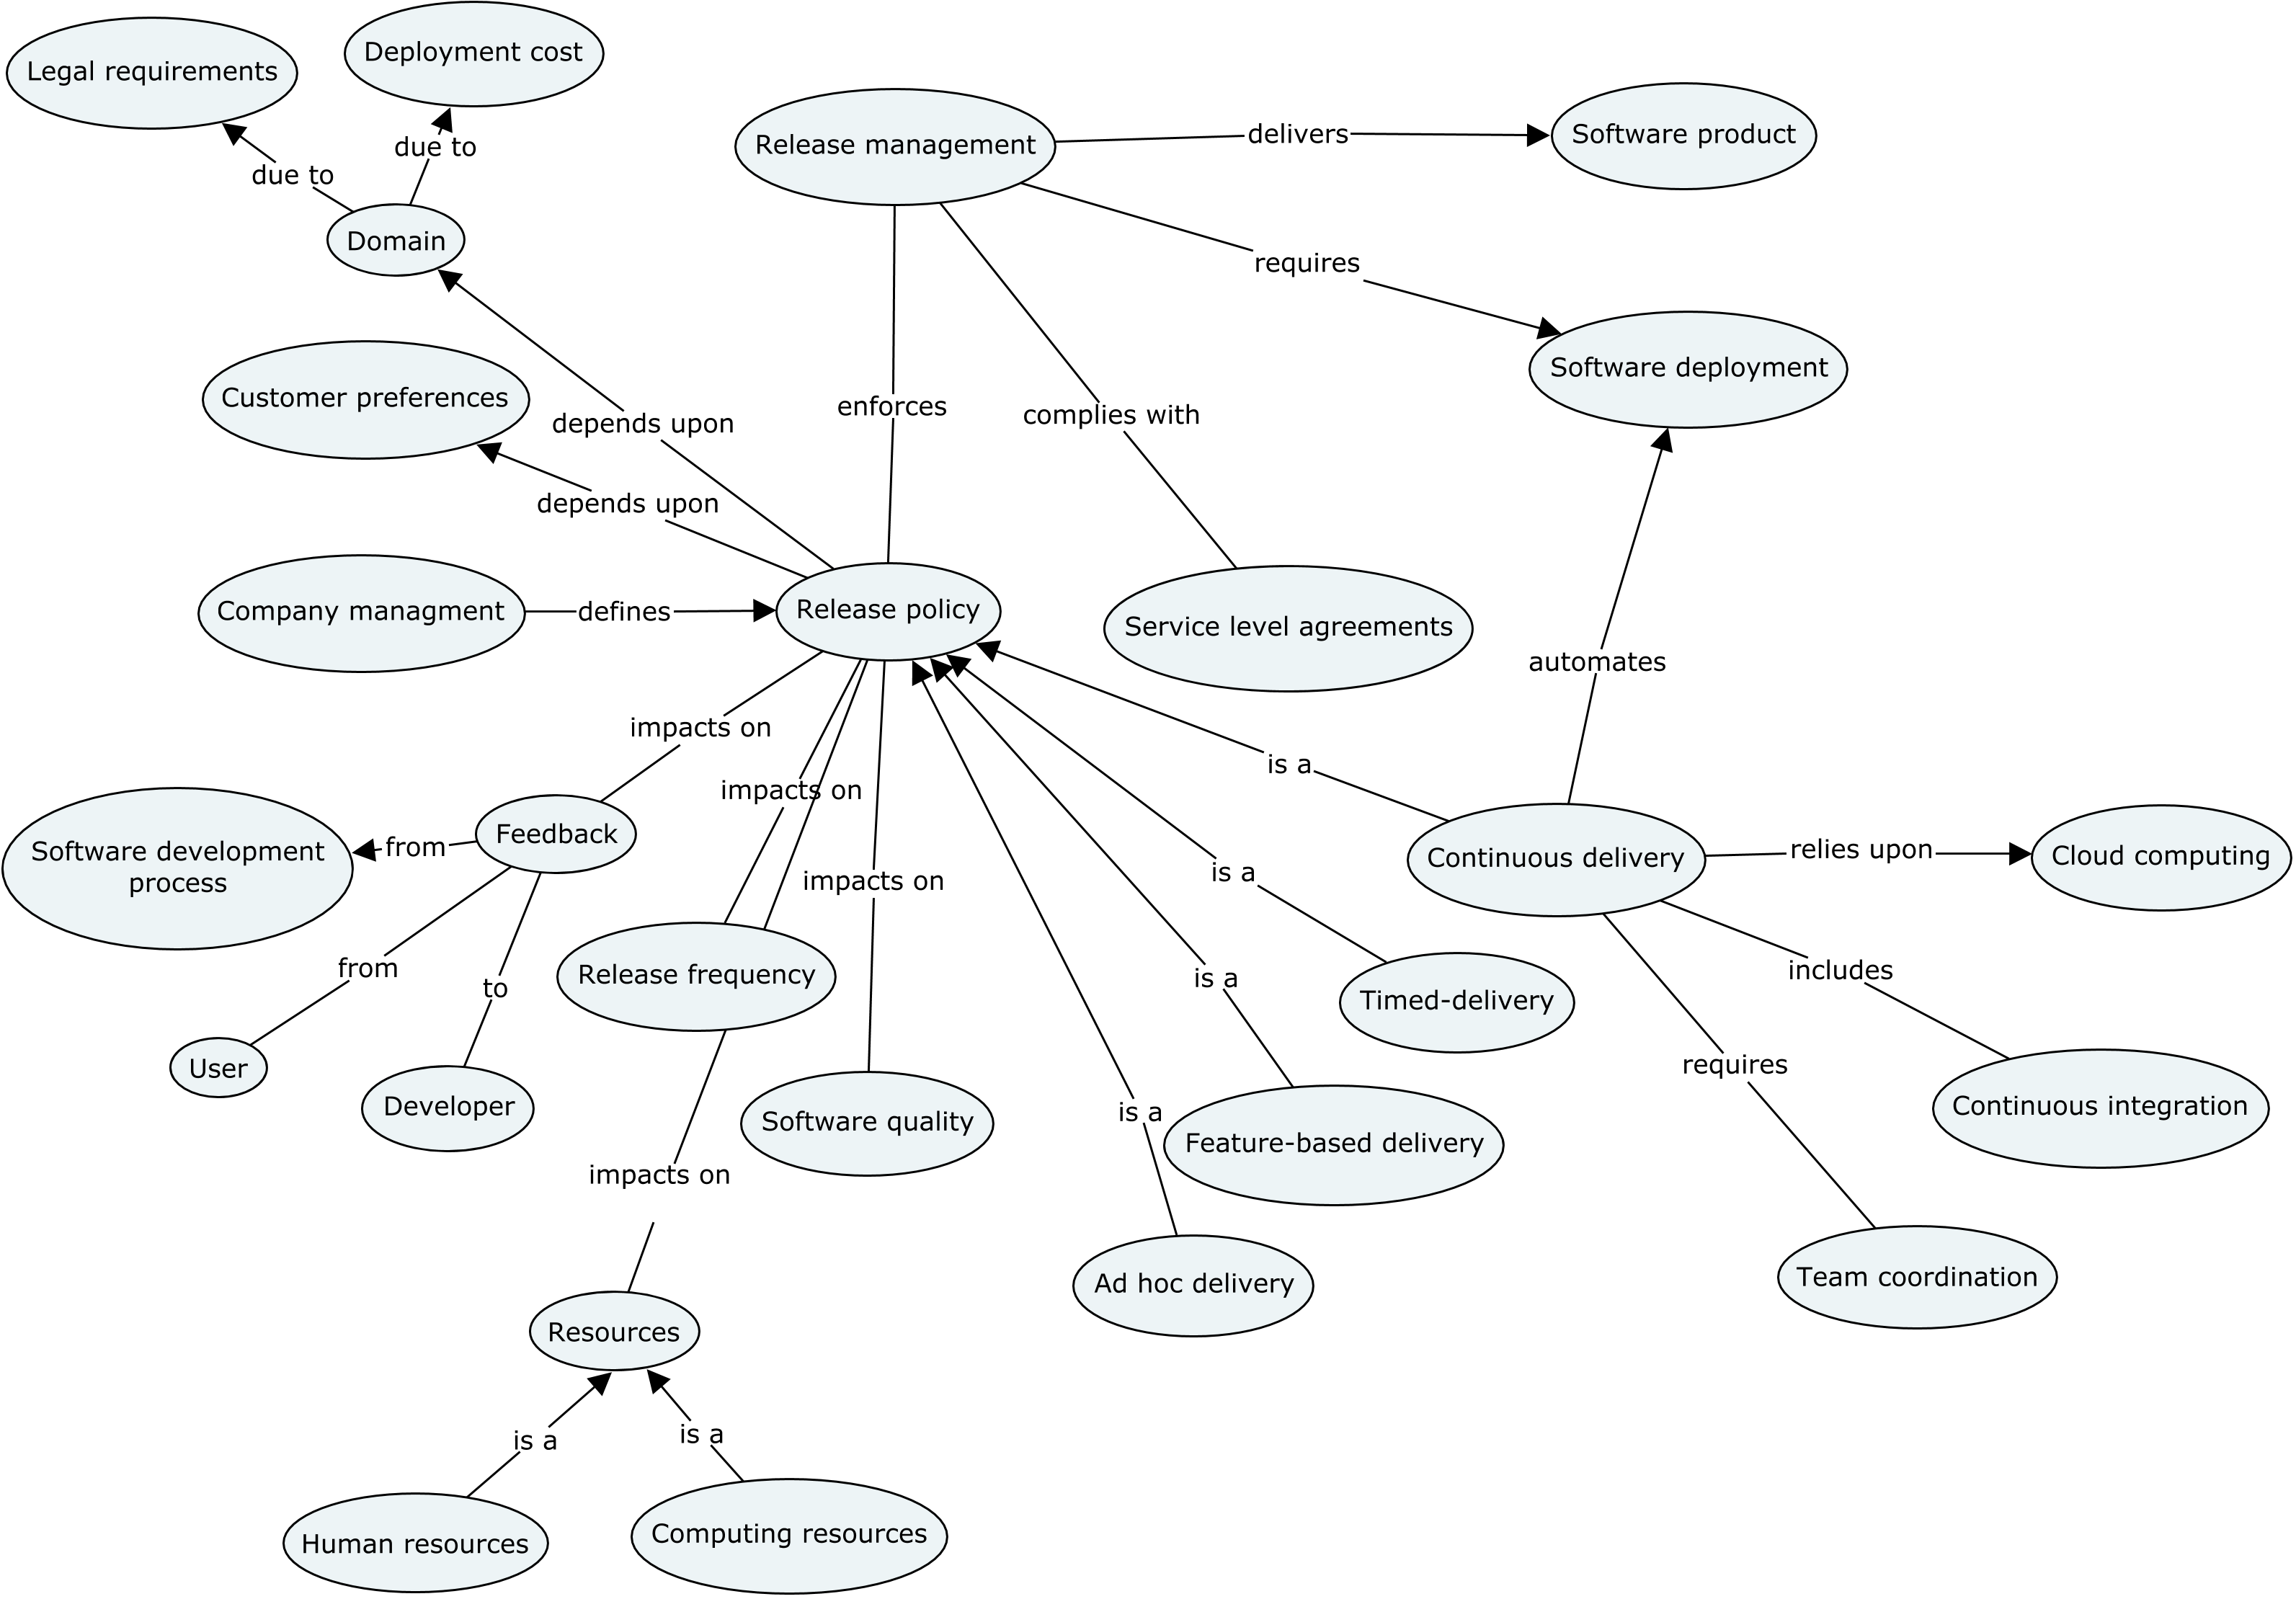
\includegraphics[width=\textwidth]{release-management}
	\end{center}
	
	\note{
		\begin{itemize}
			\item Flowing releases (lançamentos contínuos)
			\item Versões timeboxed (Ubuntu, Fedora)
			\item Atualizações constantes e ubíquas
		\end{itemize}
	}
\end{frame}



\subsection{Comunidade de desenvolvimento (OSS)}

\begin{frame}
	\frametitle{OSS}
	
	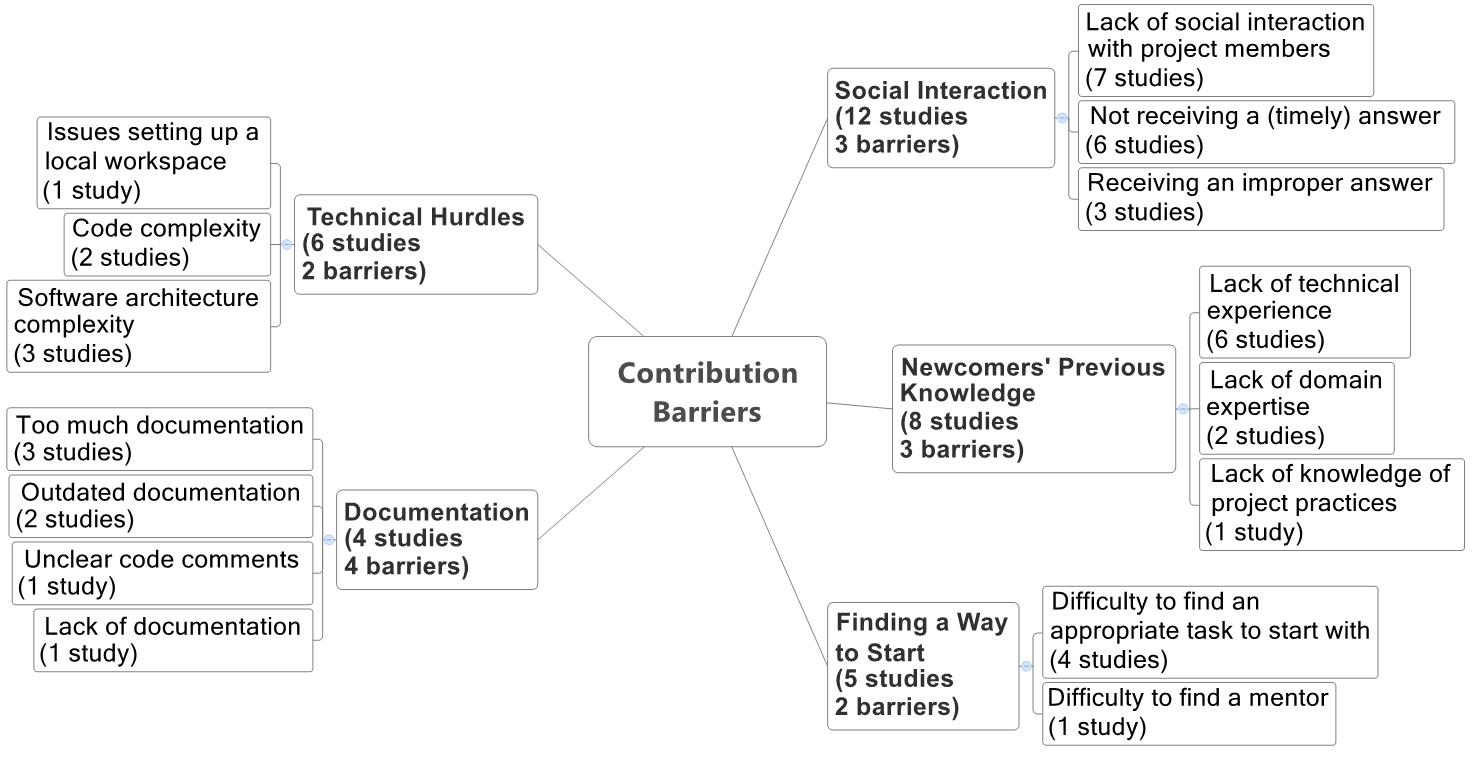
\includegraphics[width=\textwidth]{Barriers4}
	
	\note{O ``projeto de software livre'' (que, na realidade, é um produto, precisa apoiar a comunidade que o mantém.)}
\end{frame}